
\section{Introduction}
This report has been written for the Master Artificial Intelligence course Autonomous Agents. This report will contain the answers, motivation and explanation for our implementations of the tasks we had to accomplish in our third assignment for this course. These tasks were centered around the topic of `Multi-Agent Planning and Learning'.

\subsection{The environment} \label{sec:environment}
In all tasks there is assumed to be a grid world (of $11 \times 11$) with at least one predator and a prey in it. The agents can both move one tile forward each iteration. The direction they take (or if they move at all) is affected by probabilities (their policies). If they move over the edge of the grid they end up at the opposing side of the grid. We are focused on improving the decisions of all the agents, the predator(s) and the prey. 

\subsection{The state space representation} \label{sec:stateSpaceIntro}
In the experiments described the first report, we initially used a state space that was an intuitive, yet cumbersome representation. We referred to that state space representation as the `default' state space. The amount of states that was used in the default state space was $(11 \times 11) \times (11 \times 11) = 121 \times 121 = 14641$. We then changed the state space representation to a more efficient one in the second assignment, referred to as the `efficient' state space, which led to a reduction of 697 times less states, resulting in just 21 different states.
The default amount of states for this assignment would be $121^{p+1}$ for each agent, where p equals the number of predators. By using the efficient state space this has been reduced to $21\cdot 121^{p-1}$ because the prey's position is fixed in the state space representation and the predator to which this state space belongs moves along those 21 states, the rest is used to determine in which state the predator currently resides. In this assignment however the prey also learns, so to make use of our state space representation, a single predator will be used as reference point every time so that the predator is fixed at the position 0, 0 in our state space and the prey would be moving around the 21 states just like a predator. 

The reduction is increased further by pointing to the same state for each combination of current positions of the other predators, though this is only effective for more than two predators. A simple example would be a case three predators and a prey, the current predator ($p_1$) which has to find his current state would take the position of the first other predator ($p_2$) and then the position of the second other predator ($p_3$) to locate his state in the state space. In this case it shouldn't matter which position, $p_2$ or $p_3$, would be looked up first. In this case both $p_2$ then $p_3$ and $p_3$ then $p_2$ would point to the same state. This reduces the state space to:

\[
stateSpaces(p) = 
\begin{cases}
	21 & p = 1\\
    21 \cdot 121 & p = 2 \\
    \frac{21\cdot 121^{p-1}}{(p-1)!}& p > 2
\end{cases}
\]

In this assignment, we used this efficient state space representation for the learning algorithms. To give a good understanding of our learning algorithms, which were built on the efficient state space representation, we will once again explain how this representation works.

Figure \ref{fig:statespaceSymm} illustrates that there is a symmetry in the default state space, and thus that there were relatively much values redundantly computed.
By using this symmetry in the default state space a much smaller state space was achieved. 

Each state represents a distance between the prey and predator. These are represented in the lower left diagonal of a matrix, in which the $x$-axis is the relative horizontal distance in the MDP and the $y$-axis the relative vertical distance in the MDP. This matrix is shown in Figure \ref{fig:NewStateRep}. Combinations of positions of prey and predator for which the horizontal and vertical distances are equal are now treated equivalent. 
Also two combinations for which the horizontal distance in one equals the vertical distance in the other and vice versa are considered equal. In order to navigate through this state space different actions are required. These are: \textit{horizontal retreat, horizontal approach, vertical retreat, vertical approach}, as illustrated in Figure \ref{fig:statespaceSymm}, and of course the action \textit{wait}. When interacting with the environment these actions are converted into corresponding actions in the real world. This only requires the relative direction of the prey (which is always located at the centre, regardless of its coordinates) with respect to the predator. This is computed by using the difference in location of the prey and predator on the $x$- and $y$-axis.

\begin{figure}[ht]
\centering
\subfigure[The $11 \times 11$ grid divided into eight symmetric pieces, with the corresponding possible moves which are also symmetric.]{
    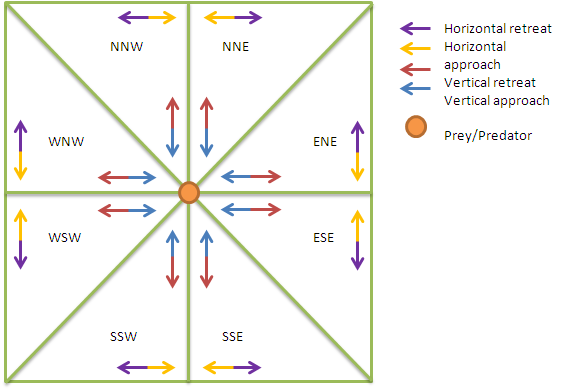
\includegraphics[width=0.5\textwidth]{statespaceSymm.png}
    \label{fig:statespaceSymm}
}
\subfigure[Colormap of $V$-values, the brighter the color the higher the corresponding $V$-value. The prey is always located on the (1, 1) coordinate in this state representation.]{
    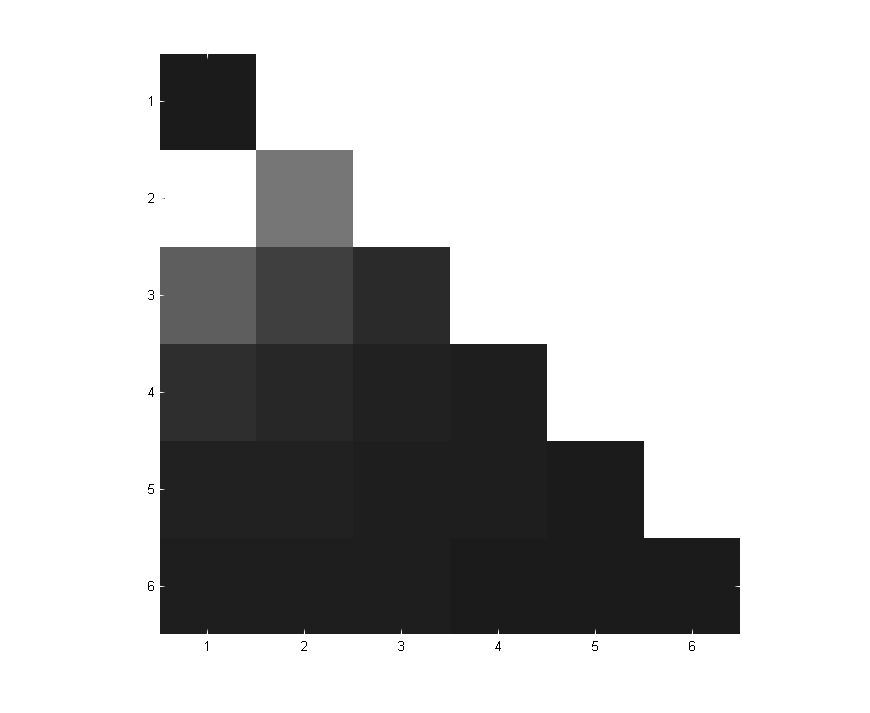
\includegraphics[width=0.4\textwidth]{VMatrixNewStateRep.png}
    \label{fig:NewStateRep}
}
\caption{Illustration of the symmetry and corresponding values of the new state space representation}
\label{fig:statespaceIll}
\end{figure}


\subsection{Implementation details}
This report will not be about our exact code and implementation details. However, a class diagram of our code is provided in Appendix \ref{app:classDiagram}.
